% Art der Arbeit: Bachelorarbeit
% Titel: "BLAST Avionics Thermal Management"
% Autor: Viktor Hoffmann
%-----------------------------------------------------------------------------------
% verwendete Packages
\documentclass{ITLR}
% Use ITLR.cls for first style-definition. 
% IMPORTANT: change in ITLR.cls colors in hyperref-package ONLY for printing; NOT for PDF submittance


% ----------- Zusätzliche Usepackages ----------------------------------------------
% Hier stehen weitere Usepackages ...
\usepackage{siunitx}
\usepackage{tikz}
\usepackage{subcaption}
\usetikzlibrary{arrows.meta}
\usepackage{acronym}

% ----------- Graphics Paths -------------------------------------------------------
\graphicspath{{Bilder/}}

%###################################################################################
% ----------- Dokumentanfang -------------------------------------------------------
\begin{document}
\setstretch{1.1667} 		% Zeilenabstand (Verhältnis, hier z.B. 14pt/12pt)
\pagestyle{Abstract}		% oben definiert

% ----------- Title & Preface  -----------------------------------------------------
\pagenumbering{Alph}
\begin{titlepage}
%---- ITLR-Logo ----
\begin{figure}[ht]
     \centering
      
\includegraphics[width=65mm]{./Logos/ITLR_Logo.eps}
\end{figure}

\hspace{200mm}

%---- Title of the study thesis ----
\begin{center}
    \begin{Large}
        Bachelorarbeit
    \end{Large}

    \vspace{2.5mm}

    \BRule
    \vspace{2.5mm}
    \begin{LARGE}
    \\
        Entwicklung des Avionik-Thermal-Managements einer Experimentalrakete
        \\
    \vspace{1mm}
    \end{LARGE}
    \vspace{2.5mm}
    \BRule
    \vspace{15mm}

    \begin{Large}

    Viktor Hoffmann \\
    
\end{Large}

\end{center}

\vfill

%---- Uni-Logo ----
\begin{wrapfigure}[4]{l}{17mm}
    
\includegraphics[width=17mm]{./Logos/unilogo_neu}
\end{wrapfigure}

\parbox[t]{120mm}
{
    \sffamily
      \vspace{3mm}
        Universität~Stuttgart\\
        \textbf{Institut~für~Thermodynamik~der~Luft-~und~Raumfahrt~(ITLR)}\\[2mm]
        Direktor: Prof.~Dr.-Ing.~habil.~Bernhard~Weigand
}




\end{titlepage}


% erste Seite: Titelblatt (wird von ITLR erstellt)
% zweite Seite: leeres Blatt
% dritte Seite: Aufgabenstellung (wird von ITLR erstellt)
% vierte Seite: Erklärung (wird von ITLR erstellt, muss aber noch unterschrieben werden)

\pagenumbering{Roman}		% Am Anfang römische Seitenzahlen
% ----------- Abstract -------------------------------------------------------------
\newpage
\phantomsection		% Korrigiert die Hyperref-Verlinkungen
\addcontentsline{toc}{chapter}{Kurzzusammenfassung} %\addcontentsline
\chapter*{Kurzzusammenfassung} % * means not in table of content
\label{chap:Kurzzusammenfassung}

% ca. 150 Worte / Aufgabenstellung, Zielsetzung, verwendete Methoden, Ergebnisse kurz vorstellen, aber nicht diskutieren / Leser entscheidet hier, ob er die Arbeit für lesenswert hält

% deutsch
Für das Projekt \ac{blast} der Hochschulgruppe \ac{hyend} wird eine neue, kompakte und hochleistungsfähige Avionik entwickelt,
die unter extremen Flugbedingungen arbeitet. Die in dieser Arbeit entwickelte Kühlung muss leicht, zuverlässig, wiederverwendbar und für eine
maximale Gehäusetemperatur von $T_\mathrm{C} \leq \SI{89.15}{\celsius}$ während der gesamte Flugdauer ausgelegt sein.
Basierend auf den Anforderungen und Flugbedingungen
wurden drei Konzepte untersucht: reiner Radiator, reines \ac{pcm} und eine hybride Radiator-\ac{pcm}-Lösung. Die Vorauslegung
ergab, dass ein Radiator wegen Aerodynamischer Aufheizung ungeeignet ist. Die hybride Lösung ist möglich, jedoch durch geometrische
Verluste und hohe Luftwärmeströme der Vorauslegung nach mit \SI{4.256}{\kilogram} schwerer als ein einfaches \ac{pcm}
mit \SI{0.347}{\kilogram}. Simulationen der Außenströmung
bestätigten trotz angenommener Vereinfachungen die Vorauslegungsergebnisse mit einer Masse des hybriden Radiator-\ac{pcm} von \SI{1.654}{\kilogram}.
Die \ac{pcm} Simulation ergab eine Überschreitung der zulässigen Temperatur.

\chapter*{Abstract} % * means not in table of content
\label{chap:Abstract}
For the \ac{blast} project of the \ac{hyend} university group, a new, compact, and high-performance avionics system is being developed to
operate under demanding flight conditions. The cooling system developed in this work must be lightweight, reliable, reusable, and designed for a maximum
case temperature of $T_\mathrm{C} \leq \SI{89.15}{\celsius}$ for the entire flightduration.
Based on the requirements and flightconditions, three concepts were investigated: pure radiator, pure \ac{pcm}, and a hybrid radiator-\ac{pcm}
solution. Preliminary design showed that a radiator is unsuitable due to aerodynamic heating. The hybrid solution is feasible but, according to
the preliminary design, heavier at \SI{4.256}{\kilogram} due to geometric losses and high convective heat flux than a simple \ac{pcm} at
\SI{0.347}{\kilogram}. Simulations of the external flow confirmed the preliminary design results despite assumed
simplifications with a mass of the hybrid radiator \ac{pcm} of \SI{1.654}{\kilogram}. The \ac{pcm} Simulation resulted in temperatures
exceeding the design requirement.

% ----------- Verzeichnisse --------------------------------------------------------
% Inhaltsverzeichnis, Abbildungsverzeichnis, Tabellenverzeichnis, Nomenklatur 
\newpage
\tableofcontents	% Erstellt automatisch die Überschrift "Inhaltsverzeichnis" mit

% Tabellenverzeichnis
\newpage
\phantomsection		% Korrigiert die Hyperref-Verlinkungen
\pagestyle{VerzeichnisseNomenklatur}		% wie oben definiert
\addcontentsline{toc}{chapter}{Tabellenverzeichnis} 	% Eintrag ins InhaltsVZ
\listoftables

% Abbildungsverzeichnis
\newpage
\phantomsection		% Korrigiert die Hyperref-Verlinkungen
\addcontentsline{toc}{chapter}{Abbildungsverzeichnis}
\listoffigures				

% Symbolverzeichnis
\newpage
\phantomsection		% Korrigiert die Hyperref-Verlinkungen
\addcontentsline{toc}{chapter}{Symbolverzeichnis}
\chapter*{Symbolverzeichnis}
	
\subsection*{Lateinische Symbole}

\begin{supertabular}{p{10mm}p{3mm}p{20mm}p{3mm}l}
$T$ && \SI{}{\kelvin} && Temperatur\\
$c$ && \SI{}{\joule\per\kilogram\per\kelvin} && Spezifische Wärmekapazität\\
$h$ && \SI{}{\joule\per\kilogram} && Spezifische Schmelzenthalpie\\
$Q$ && \SI{}{\joule} && Wärme\\
$\dot{Q}$ && \SI{}{\watt} && Wärmestrom\\
$\dot{q}$ && \SI{}{\watt\per\meter\squared} && Wärmestromdichte\\ 
$m$ && \SI{}{\kilo\gram} && Masse\\
$A$ && \SI{}{\meter\squared} && Fläche\\
$S$ && \SI{}{\newton\per\meter\cubed} && Quellterm\\
$R$ && \SI{}{\kelvin\per\watt} && Wärmeleitwiederstand\\
\end{supertabular}


\subsection*{Griechische Symbole}

\begin{supertabular}{p{10mm}p{3mm}p{20mm}p{3mm}l}
$\rho$ && \SI{}{\kilogram\per\cubic\meter} && Dichte\\
$\lambda$ && \SI{}{\watt\per\meter\per\kelvin} && Wärmeleitfähigkeit\\
$\gamma$ && \SI{}{\per\kelvin} && Flüssigkeitsanteil\\
$\beta$ && && Wärmeausdehnungskoeffizient\\
$\varepsilon$ && && Emissionsgrad\\
$\alpha$ && && Absorptionsgrad\\
$\nabla$ && && Nablaoperator\\
\end{supertabular} 

\subsection*{Indizes}

\begin{supertabular}{p{10mm}p{3mm}p{20mm}p{3mm}l}
solidus && && Solidus Punkt des Phasenwechsels\\
liquidus && && Liquidus Punkt des Phasenwechsels\\
solid && && Feststoff Eigenschaften\\
liquid && && Flüssigstoff Eigenschaften\\
fus && && Schmelz Phasenwechsel\\
safety && && Mit Sicherheitsfaktor 1.5\\
senke && && Wärmesenke\\
total && && Totalgröße\\
ges && && Gesamt\\
p && && Konstanter Druck\\
J && && Sperrschicht\\
C && && Gehäuse\\
f && && Freistrom\\
w && && Wand\\
t && && Spektral integriert\\
s && && Solar\\
x && && Lokale Größe\\
r && && Recovery Größe\\
a && && adiabat\\
\end{supertabular} 

\subsection*{Konstanten}

\begin{supertabular}{p{10mm}p{3mm}p{50mm}p{3mm}l}
$\sigma$ && \SI{5.67e-8}{\watt\per\meter\squared\per\kelvin\tothe{4}} && Stefan-Boltzmann-Konstante\\
$\kappa$ && \SI{1.40}{} && Isentropenexponent der Luft\\
$\eta_0$ && \SI{18.27e-6}{\pascal\second} && Sutherlands-Formel Referenzviskosität\\
$T_0$ && \SI{291.15}{\kelvin} && Sutherlands-Formel Referenztemperatur\\
$C$ && \SI{120}{\kelvin} && Sutherland Konstante\\
\end{supertabular}

\newpage

%---Akronyme
\subsection*{Abkürzungen}
\begin{acronym}[BLAST]
\acro{pcm}[PCM]{Phase Change Material}
\acro{pcb}[PCB]{Printed Circuit Board}
\acro{blast}[BLAST]{Biliquid launch and Space Technology}
\acro{fcc}[FCC]{Flight Control Computer}
\acro{hyend}[HyEnD]{Hybrid Engine Development}
\acro{cfd}[CFD]{Computational Fluid Dynamics}
\acro{cht}[CHT]{Conjugate Heat Transfer}
\acro{pgs}[PGS]{Pyrolithic Graphite Sheet}
\acro{maxq}[max~Q]{Maximaler dynamischer Druck}
\acro{gse}[GSE]{Ground Support Equipment}
\acro{pcdu}[PCDU]{Power Control and Delivery Unit}
\acro{atm}[ATM]{Avionik-Thermal-Management}
\acro{rom}[ROM]{Reduced Order Model}
\acro{udf}[UDF]{User Defined Function}
\end{acronym}

% ----------- Verzeichnisse Ende-----------------------------------------------------
\newpage
\pagestyle{main}			% ab hier: normale Kopf- und Fußnoten
% ----------- Einleitung ------------------------------------------------------------
\chapter{Einführung}			
\label{sec:Introduction}
\pagenumbering{arabic}		%ab hier: arabische Seitenzahlen (Hauptteil)

% Problemstellung und Lösungsansätze, 2-3 Seiten / keine Ergebnisse & Folgerungen /

Die Avionik ist ein Grundstein jeder erfolgreichen Experimentalrakete. Ob es hierbei um Telekommunikation,
Datenerfassung oder auch aktive Steuerung und Regelung von
Instrumenten und dem Fahrzeug während des Flugs geht, kompakte Hochleistungsmikroelektronik ist immer gefragt und muss oft redundant ausgeführt sein.
Diese Elektronik, die zudem noch extremen Bedingungen ausgesetzt wird, kommt jedoch mit einer
substanziellen Wärmeleistung und Wärmestromdichte die bei mangelhafter Rücksicht zu reduzierter Lebensdauer der Avionik führt
oder sogar die Mission frühzeitig scheitern lässt.

Diese Arbeit befasst sich mit dem Lösungsansatz des dargestellten Problems für das Projekt \ac{blast} der studentischen Hochschulgruppe \ac{hyend},
wo eine neue Avionik entwickelt und ein \ac{atm} benötigt wird.

\section{Darstellung des Problems}

Das Thermal-Problem einer Experimentalrakete beginnt bereits lange vor dem eigentlichen Start. Oft muss nach Integration und
Befestigung der Rakete auf der Startvorrichtung und Verbindung mit dem \ac{gse} noch einige Stunden auf das Startfenster gewartet werden.
Während dieser Zeit steht die Rakete der Umwelt ausgesetzt in der Sonne und kann je nach Bedingungen 
unzulässige Temperaturen für die Elektronik erreichen. Da in dieser Phase eine Verbindung mit dem 
\ac{gse} besteht, kann Masse durch externe Kühlung währenddessen eingespart werden, weshalb in dieser Arbeit nur für die darauf folgende 
Flugphase das \ac{atm} entwickelt werden soll.
Da \ac{blast} für ein Apogäum über der Kármán-Linie (\SI{100}{\kilo\meter} über dem Meeresspiegel) entwickelt wird, sind während des Fluges extreme Umweltbedingungen
durch aerodynamische Aufheizung, Mikrogravitation und annäherndes Vakuum zu erwarten, die ein robustes \ac{atm} fordern.

In der Vergangenheit wurde bei \ac{hyend} oft die Avionik ohne Redundanz oder zusammen mit fertig gekaufter Avionik für 
missionskritische Aufgaben wie den Fallschirm-Auswurf ausgeführt. Beim Projekt \ac{blast} soll das vermieden werden, 
indem der selbst entwickelte \ac{fcc} in Dual-Duplex-Redundanz ausgelegt wird. Dementsprechend gibt es vier Computer, die
die selben Programme ausführen und den vierfachen Stromverbrauch gegenüber einfach ausgeführter Avionik haben. Hinzu kommen
weitere Kameras, Funkplatinen, Verstärker, Sensorplatinen etc., die jedoch keine redundante Ausführung haben.

\section{Zielsetzung der Arbeit}

Da es sich beim \ac{atm} um ein unterstützendes Subsystem handelt, soll besonders hohe Zuverlässigkeit gewährleistet werden, da trotz der
Redundanz des \ac{fcc} ein Ausfall der Kühlung zum Ausfall durch Überhitzung führen kann.
Des Weiteren ist Wiederverwendbarkeit, Kosten minimieren und besonders komplexe Integrations- und Vorbereitungsvorgänge
vermeiden eine Priorität.
Als letzte Anforderung soll wegen des begrenzten Massenbudgets der Avionik
besonders auf Leichtbau geachtet werden und die Masse des \ac{atm} soweit wie möglich minimiert werden.

\section{Lösungsweg}

Um ein geeignetes \ac{atm} zu entwickeln wird zunächst eine Auswahl an etablierten Lösungen aus der Luft- und Raumfahrtindustrie
getroffen, die die gestellten Anforderungen erfüllen können.

Diese werden in der Vorauslegung mithilfe eines \ac{rom} in Python ausgewertet, das eine dimensionsreduzierte Näherung des nichtlinearen Referenzmodells liefert, um eine erste Abschätzung der Leistungsfähigkeit zu erhalten.
Anschließend wird die Vorauslegung, soweit mit vorhandenen Rechenressourcen möglich, durch \ac{cht}-Simulationen mit Domänenreduktion
überprüft und mit diesen Ergebnissen verglichen.

%----------- Literaturrecherche -----------------------------------------------------
\newpage
\chapter{Grundlagen}
\label{chap:Grundlagen}			% durch \label{} später auf Element verweisen

In diesem Kapitel werden die Thermodynamischen, Chemischen und Numerischen Grundlagen die in dieser Arbeit angewandt wurden aufgelistet
und erläutert.
% Bücher, aber auch Paper etc. 

\section{Sensible Wärme}\label{sec:sensiblewaerme}
Unter sensibler Wärme versteht man die Eigenschaft von Masse durch eine Temperaturänderung Wärmeenergie zu absorbieren oder abzugeben. Dieses
Phänomen kann durch die Änderung der kinetischen Energie von den molekularen Teilchen im System erklärt werden. Durch das Einführen von
Wärmeenergie in ein System steigt die kinetische Energie der Teilchen:

\begin{equation}
    c = \frac{\Delta Q}{m \cdot \Delta T}
\end{equation}

$c$ beschreibt die spezifische Wärmekapazität, welche entweder bei konstantem Druck oder konstantem Volumen angegeben ist,
$Q$ ist die Wärmeenergie, $m$ die Masse und $T$ die Temperatur

Da Elektronik eine gewisse Eigenmasse hat und meist Teil einer größeren Baugruppe ist, gibt es durch die sensible Wärme eine Dämpfung
zu Temperaturänderungen, welche jedoch zeitlich von der Wärmeleitfähigkeit der Materialien abhängt.

\section{Latente Wärme}\label{sec:latentewaerme}

Im Gegenteil zur sensiblen Wärme ist latente Wärme, auch Umwandlungsenthalpie genannt, die Eigenschaft von Masse bei einem Phasenwechsel Wärmeenergie
zu absorbieren oder abzugeben, ohne dass sich dabei die Temperatur ändert. Das ist durch die Erhöhung der potentiellen Energie der Teilchen,
statt der kinetischen wie bei der sensiblen Wärme, zu verstehen. Effektiv erhöht sich die potentielle Energie durch Änderung der Bindungszustände.
Die Stoffkonstante der Umwandlungsenthalpie ist die spezifische Umwandlungsenthalpie $h$:

\begin{equation}
    h = \frac{\Delta Q}{m}
\end{equation}

Zu beachten ist, dass die Konvention der Schreibweise für die massenspezifische Fest-Flüssig Umwandlungsenthalpie spezifische Schmelzenthalpie ist,
aber für die massenspezifische Flüssig-Gas Umwandlungsenthalpie nur Verdampfungsenthalpie ist.

Die latente Wärme ist für die meisten Materialien im Fest-Flüssig Übergang um mindestens den Faktor 10 größer als die sensible Wärme bei
einem Grad Temperaturerhöhung. Genauso ist die Verdampfungsenthalpie vom Flüssig-Gas Übergang meist um etwa den Faktor 10 größer als die 
spezifische Schmelzenthalpie~\cite{fusion-vaporization}.

\section{Wärmeübertragung}\label{sec:waermeuebertragung}

Um Wärme innerhalb von einem System günstig zu verteilen, oder die Energie aus dem System zu entfernen, gibt es drei Mechanismen.

\subsection{Wärmestrahlung}\label{sec:strahlung}

Bei der Wärmestrahlung geben Teilchen beim aufnehmen oder abgeben kinetischer Energie eine Gewisse Menge an Energie in Form
von Elektromagnetischer Strahlung ab. Da die Strahlungsleistung von der vierten Potenz der Temperatur
abhängt, ist dieser Modus erst bei sehr hohen Temperaturen dimensionierend, kann jedoch im Vakuum dominant sein:

\begin{equation}
    \label{eq:radiation}
    \dot{Q}=\sigma\varepsilon A T^{4}
\end{equation}

$\dot{Q}$ ist der Wärmestrom, $\sigma$ die Stefan-Boltzmann-Konstante, $\varepsilon$ der Emissionsgrad, welcher von der Wellenlänge
abhängt, $A$ die Fläche und $T$ die Temperatur des Radiators.

\subsection{Wärmeleitung}\label{sec:waermeleitung}

Bei der Wärmeleitung wird Wärmeenergie in einem Körper durch diffusion der kinetischen Energie der Teilchen verteilt.
Die Wärmestromdichte $\dot{q}$ in einem Temperaturgradienten wird durch das Fourier-Gesetz beschrieben:

\begin{equation}
  \label{eq:fourier}
  \vec{\dot{q}} = -\lambda \nabla T
\end{equation}

Hier ist $\lambda$ die Wärmeleitfähigkeit des Materials.
Für eine eindimensionale Wand ergibt sich die Gleichung mit der Querschnittfläche $A$ und der Dicke $\Delta x$ zu:

\begin{equation}
  \label{eq:fourier_1d}
  \dot{Q} = \lambda A \frac{\Delta T}{\Delta x}
\end{equation}

Der Wärmeleitwiederstand $R$ für einen Körper lässt sich durch die Temperaturdifferenz pro Watt definieren:

\begin{equation}
  \label{eq:waermewiederstand}
  R = \frac{\Delta T}{\dot{Q}}
\end{equation}

\subsection{Konvektion}\label{sec:konvektion}

Bei der Konvektion wird Wärmeenergie durch Massenaustausch transportiert. Bei der erzwungenen Konvektion bekommt das Fluid durch äußere Kräfte
eine relative Geschwindigkeit, die zum Massenaustausch führt. Andererseits resultiert bei der natürlichen Konvektion nur die eigene
inhomogene Temperaturverteilung, durch beispielsweise eine anliegende heiße Wand, zu einem Temperaturanstieg und infolge dessen zu einem
Dichteanstieg, der in einem Beschleunigungsfeld zu Auftriebskräften und automatischer Bewegung des Fluids führt.
Für den Wärmeübergang zwischen Fluid und Festkörper ergibt sich:

\begin{equation}
    \dot{Q}=\alpha A \Delta T 
\end{equation}

Hier ist $\alpha$ der Wärmeübergangskoeffizient.
Für den spezifischen Wärmestrom zwischen Fluid und Wand folgt daraus:

\begin{equation}
  \label{eq:qdot_freestream}
  \dot{q} = \alpha \ (T_{\infty} - T_\text{w})
\end{equation}

Der Wärmeübergangskoeffizient $\alpha$ kann aus der Nußelt-Beziehung für Längsangeströmte ebene Platte genommen. Diese lautet
für laminare Grenzschichten im Gültigkeitsbereich $\text{Re} < \text{Re}_k \left(\text{Re}_k \approx 5 \cdot 10^5\right)$ und $0,6 \leq \text{Pr} \leq 2000$:

\begin{equation}
  \label{eq:nusselt_laminar}
  \text{Nu}_x = \frac{\alpha_x x}{\lambda} = \num{0,332} \ \text{Pr}^{\frac{1}{3}} \ \text{Re}_x^{\frac{1}{2}}
\end{equation}

für turbulente Grenzschichten mit Gültigkeitsbereich: $5 \cdot 10^5 \leq \text{Re}_L \leq 10^7$ und $ 0,6 \leq \text{Pr} \leq 2000$ lautet die Gleichung:

\begin{equation}
  \label{eq:nusselt_turbulent}
  \text{Nu}_x = \frac{\alpha_x x}{\lambda} = \num{0,0296} \ \text{Re}_x^{0,8} \ \text{Pr}^{\frac{1}{3}}
\end{equation}

Für die Reynolds-Zahl und Prandtl-Zahl werden die folgenden zwei Gleichungen verwendet:

\noindent\begin{minipage}{.5\linewidth}
  \begin{equation}
    \label{eq:reynolds}
    Re_x = \frac{U \rho x}{\eta}
  \end{equation}
\end{minipage}%
\begin{minipage}{.5\linewidth}
  \begin{equation}
    \label{eq:prandtl}
    Pr = \frac{c_p \eta}{\lambda}
  \end{equation}
\end{minipage}

Die Dynamische Viskosität $\eta$ wird mittels der Sutherlands-Formel berechnet, wobei $\eta_0$, $C$ und $T_0$ Konstanten für Luft sind:

\begin{equation}
  \label{eq:dynamische_viskositaet}
  \eta = \eta_0 \frac{T_0 + C}{T_{\infty} + C} {\left( \frac{T_{\infty}}{T_0} \right)}^{\frac{3}{2}}
\end{equation}

Eine Strömung ist im Überschallbereich, wenn ihre Machzahl größer als 1 ist:

\begin{equation}
  \label{eq:machzahl}
  Ma = \frac{U}{a}
\end{equation}

Wobei $U$ die Strömungsgeschwindigkeit und $a$ die lokale Schallgeschwindigkeit ist. Im Überschallbereich treten verschiedene
Effekte durch die Kompressibilität der Strömung auf, wie etwa durch Stoßwellen mit sprunghaftem Anstieg von Temperatur und Druck,
oder Expansionsfächern mit sprunghaftem Abfall dieser Größen. Auch die adiabate Kompression resultiert in Temperaturerhöhungen.
Die in einer Grenzschicht erreichte Temperatur durch Reibung
ist immer kleiner als die Totaltemperatur $T_{\infty} < T_r < T_\mathrm{total}$, da die kinetische Energie nur teilweise in innere Energie
umgewandelt wird und somit mit dem Recovery-Faktor $r$ skaliert ist:

\begin{equation}
  \label{eq:recovery_temperatur}
  T_r = T_{\infty} \left( 1 + r \frac{\kappa - 1}{2} \text{Ma}^2 \right)
\end{equation}

Der Recovery-Faktor kann mittels der folgenden Gleichung berechnet werden:

\begin{equation}
  \label{eq:recovery_faktor}
  r = \frac{2}{\left( \kappa - 1 \right) \mathrm{Ma_{\infty}}^2} \left( \frac{T_\mathrm{a_{w}}}{T_{\infty}} - 1 \right) \approx
  \begin{cases}
    \sqrt[3]{\text{Pr}} & \text{für turbulente Grenzschicht}\\
    \sqrt{\text{Pr}} & \text{für laminare Grenzschicht}
  \end{cases}
\end{equation}

In einer kompressiblen Strömung bei $\mathrm{Ma} > 0.3$ wird somit $T_{\infty}$ aus \ref{eq:qdot_freestream} zu $T_\text{r}$:

\begin{equation}
  \label{eq:qdot_recovery}
  \dot{q} = \alpha \ (T_r - T_w)
\end{equation}

\section{Simulation}
\section*{Aerodynamische Aufheizung}

Die numerische Strömungssimulation (\ac{cfd}) ist ein Verfahren zur Berechnung von Strömungs- und Wärmeübergangsprozessen
mithilfe numerischer Methoden. \ac{cfd} erlaubt die Untersuchung komplexer Geometrien und Betriebsbedingungen,
die experimentell nur schwer oder gar nicht möglich sind. Ziel ist es, die Navier-Stokes-Gleichungen in differentieller Form auf einer
diskreten Gitterstruktur zu lösen. Diese Erhaltungsgleichungen sind die Massenerhaltung:

\begin{equation}
  \label{eq:navier_massenerhaltung}
  \frac{\partial \rho}{\partial t} + \nabla \left( \rho \vec{u} \right) = 0
\end{equation}

Impulserhaltung:

\begin{equation}
  \label{eq:navier_impulserhaltung}
  \frac{\partial \left( \rho \vec{u} \right)}{\partial t} + \nabla \left( \rho \vec{u} \vec{u} \right) = -\nabla p + \nabla \tau + \rho \vec{g}
\end{equation}

und Energieerhaltung:

\begin{equation}
  \label{eq:navier_energieerhaltung}
  \frac{\partial \left(\rho \vec{u}\right)}{\partial t} + \nabla \left[\left(\rho E + p\right)\vec{u}\right] = \nabla \left(k \nabla T\right) + \Phi
\end{equation}

Hier sind $\rho$ die Dichte, $\vec{u}$ der Geschwindigkeitsvektor, $p$ der statische Druck, $\tau$ der Spannungstensor,
$\vec{g}$ die Gravitationsbeschleunigung, $E$ die spezifische Gesamtenergie, $T$ die Temperatur, $k$ die Wärmeleitfähigkeit
und $\Phi$ der viskose Dissipationsterm.

Eine wichtige Metrik bei der Behandlung von Grenzschichten in viskosen Fluiden ist der Dimensionslose Wandabstand:

\begin{equation}
  \label{eq:yplus}
  y^+ = \frac{\rho u_{\tau} y}{\eta}
\end{equation}

Dieser wird mittels des Abstandes $y$ der ersten Zelle die an der Wand anliegt, der Schubspannung an der Wand $\tau_w$ und der daraus resultierenden Schubspannungsgeschwindigkeit $u_{\tau}$ berechnet:

\noindent\begin{minipage}{.5\linewidth}
  \begin{equation}
    \label{eq:schubspannung}
    \tau_w = \eta \left.\frac{\partial u}{\partial y}\right|_{y=0} = \frac{1}{2} \rho U_{\infty}^{2} C_f
  \end{equation}
\end{minipage}%
\begin{minipage}{.5\linewidth}
  \begin{equation}
    \label{eq:schubspannung_geschwindigkeit}
    u_{\tau} = \sqrt{\frac{\tau_w}{\rho}}
  \end{equation}
\end{minipage}

Hierbei ist $\eta$ die dynamische Viskosität, $\left.\frac{\partial u}{\partial y}\right|_{y=0}$ der Geschwindigkeitsgradient senkrecht zur Wand
und $C_f$ der Reibungsbeiwert.
Für $C_f$ gibt es folgende empirische Näherungen~\cite{Anderson-2017}:

\begin{minipage}{.5\linewidth}
  \begin{equation}
    \label{eq:reibungsbeiwert_laminar}
    C_f \approx \frac{0.664}{\sqrt{{Re}_x}} \hspace{0.5em} \mathrm{bei} \hspace{0.5em} Re \leq \SI{5e5}{}
  \end{equation}
\end{minipage}%
\begin{minipage}{.5\linewidth}
  \begin{equation}
    \label{eq:reibungsbeiwert_turbulent}
    C_f \approx \frac{0.0592}{{Re}_x^{1/5}} \hspace{0.5em} \mathrm{bei} \hspace{0.5em} Re > \SI{5e5}{}
  \end{equation}
\end{minipage}

Für Wärmeübertragungsprobleme an Wänden muss man die Zellhöhe so wählen, dass man im Bereich $y^+ \leq 1$ bleibt.

\section*{PCM}
Um Temperatur- und Phasenabhängige Eigenschaften für die \ac{cht}-Simulation von \ac{pcm} darzustellen, sowie Zeitabhängige Auftriebsterme, kommen weitere Modelle dazu,
die in ANSYS Fluent nicht implementiert sind. Dafür wird eine in C programmierte \ac{udf} verwendet, die in Fluent direkt importiert
und kompiliert werden kann.
Die Boussinesq-Approximation modelliert den Auftrieb infolge von geringen Dichteänderungen. Für den Auftrieb
in dem Impulsterm ergibt sich somit~\cite{akamcae-udf}:

\begin{equation}
  \label{eq:udf_bouss}
  S = -\rho_0 \, g_\text{eff}(t)\,\beta\,(T-T_0)
\end{equation}

Hierbei ist $S$ der Quellterm, $\beta$ der Wärmeausdehnungskoeffizient, $g_\text{eff}(t)$ die effektive, Zeitabhängige Beschleunigung,
$T_0$ und $\rho_0$ die Referenz-Temperatur und Dichte. Diese Approximation kann den Rechenaufwand erheblich verringern und ist für folgende Bedingungen gültig:

\noindent\begin{minipage}{.5\linewidth}
  \begin{equation}
    \label{eq:bossinesque_bedingung1}
    \frac{\Delta T}{T_0} \ll 1
  \end{equation}
\end{minipage}%
\begin{minipage}{.5\linewidth}
  \begin{equation}
    \label{eq:bossinesque_bedingung2}
    \text{Ma} \ll 1
  \end{equation}
\end{minipage}

ANSYS Fluent verwendet zur Modellierung des Schmelzbereiches ein internes \allowbreak Enthalpy-Porosity-Modell, welches das \ac{pcm} als poröses Material
mit diskreter Fest- und Flüssigphase ansieht. Hierfür ist die Dichte $\rho$ notwendig und kann in Abhängigkeit des Flüssigkeitsanteils $\gamma$ berechnet werden.
Zwischen der Dichte der Flüssig- und Feststoffphase wird linear interpoliert~\cite{akamcae-udf}:

\begin{equation}
  \label{eq:udf_dichte}
  \rho(\gamma) = \left(1- \gamma\right) \rho_\text{solid} + \gamma \rho_\text{liquid} \qquad \gamma \in [0,1]
\end{equation}

Die spezifische Wärmekapazität ergibt sich im Schmelzbereich durch eine Dichtegewichtete Mischung~\cite{akamcae-udf}:

\begin{equation}
  \label{eq:udf_cp}
    c_p(T)=
  \begin{cases}
    c_{p,\mathrm{solid}}, & T < T_\mathrm{solid},\\[6pt]
    \dfrac{(1-\gamma)\,\rho_\mathrm{solid}\,c_{p,\mathrm{solid}} + \gamma\,\rho_\mathrm{liquid}\,c_{p,\mathrm{liquid}}}
          {(1-\gamma)\,\rho_\mathrm{solid} + \gamma\,\rho_\mathrm{liquid}}, & T_\mathrm{solid} \le T \le T_\mathrm{liquid},\\[12pt]
    c_{p,\mathrm{liquid}}, & T > T_\mathrm{liquid}.
  \end{cases}
\end{equation}

Die Wärmeleitfähigkeit $\lambda$ im Schmelzbereich hingegen lässt sich direkt berechnen~\cite{akamcae-udf}:

\begin{equation}
  \label{eq:udf_lambda}
  \lambda(\gamma)= (1-\gamma)\,\lambda_{\mathrm{solid}} + \gamma\,\lambda_{\mathrm{liquid}}
\end{equation}

Die Dynamische Viskosität $\eta$ wird hier, anders als für Luft in der Vorauslegung \ref{eq:dynamische_viskositaet}, mittels eines empirischen
Polynomfit~\cite{akamcae-udf} abhängig von der Temperatur berechnet:

\begin{equation}
  \label{eq:udf_mu}
  \eta(T)= \left(9\times 10^{-4}\,T^{2} - 0.6529\,T + 119.94\right)\times 10^{-3}
\end{equation}

In der verwendeten Software ANSYS Fluent werden diese Gleichungen über die Finite-Volumen-Methode gelöst. Dabei werden die Erhaltungsgleichungen
über diskrete Kontrollvolumina integriert, wodurch für jede Zelle ein algebraisches Gleichungssystem entsteht. Dieses
wird iterativ gelöst, bis vorgegebene Konvergenzkriterien erfüllt sind.

% ----------- Methodik --------------------------------------------------------------
\chapter{Methodik}
\label{chap:Methodik}
% Ziel hier: den Leser in die Lage versetzen, die wesentliche Struktur der Arbeit nachvollziehen zu können (Vorgehen / Geräte / Materialien / Verfahren [also auch Software]  / getroffene Annahmen ... sollten hier erklärt werden)
\section{PCM}\label{sec:pcm}

Die Thermodynamischen Eigenschaften von Eicosane, aufgeführt in Tabelle \ref{tab:eicosane_data}, wurden aus mehreren Quellen entnommen.\\

\begin{table}[H]
  \centering
  \caption{Stoffdaten für Eicosane~\cite{NIST,Nazarychev-2022,Benbrika-2020,Stryker-1990}}\label{tab:eicosane_data}
  \begin{tabular}{l|l}
    \hline
    $T_{\text{solidus}}$ & \SI{309}{\kelvin} \\
    \hline
    $T_{\text{liquidus}}$ & \SI{311}{\kelvin} \\
    \hline
    $c_{p,\text{liquid}}$ & \SI{2350.05}{\joule\per\kilogram\per\kelvin} \\
    \hline
    $c_{p,\text{solid}}$ & \SI{2132.4}{\joule\per\kilogram\per\kelvin} \\
    \hline
    $\rho_{\text{solid}}$ & \SI{910}{\kilogram\per\cubic\meter} \\
    \hline
    $\rho_{\text{liquid}}$ & \SI{769}{\kilogram\per\cubic\meter} \\
    \hline
    $\lambda_{\text{liquid}}$ & \SI{0.1505}{\watt\per\meter\per\kelvin} \\
    \hline
    $\lambda_{\text{solid}}$ & \SI{0.4248}{\watt\per\meter\per\kelvin} \\
    \hline
    $\gamma$ & \SI{0.0009}{\per\kelvin} \\
    \hline
    $h_{\text{fus}}$ & \SI{240998.86}{\joule\per\kilogram} \\
    \hline
  \end{tabular}
\end{table}

\begin{figure}[H]
    \centering
    \begin{subfigure}{0.9\textwidth}
        \centering
        \includegraphics[width=\linewidth]{../../Code/pcm_mass.pdf}
        \caption{PCM Masse}\label{fig:pcm_mass}
    \end{subfigure}
    \vspace{1em}  % Optional vertical spacing
    \begin{subfigure}{0.9\textwidth}
        \centering
        \includegraphics[width=\linewidth]{../../Code/pcm_heat_capacity.pdf}
        \caption{PCM Wärmeaufnahme}\label{fig:pcm_heat}
    \end{subfigure}
    \caption{PCM Auslegung}\label{fig:pcm_mass_heat}
\end{figure}

\newpage

\section{Radiator}\label{sec:Radiator}

Hier steht was zu Radiatoren.

\begin{figure}[H]
  \centering
  \includegraphics[width=\linewidth]{../../Code/radiator_leistung.pdf}
  \caption{Radiator Leistung nach Fläche und Temperatur}\label{fig:pcm_heatflux}
\end{figure}

\newpage

\section{PCM-Radiator-Hybrid}\label{sec:pcmRadiatorHybrid}

Eine Hybridlösung wird auch in erwägung gezogen, um die Masse durch Nutzung eines Radiators zu minimieren, wobei wegen aerodynamischer Aufheizung für kurze Zeit ein PCM gebraucht werden könnte.
Um eine umständliche Simulation mittels \ac{cfd} zu vermeiden, wird die Außenkontour der Rakete von Spitze bis Avionik-Sektion, mit Hilfe der Nußelt-Beziehungen, als längsangeströmte ebene Platte angesehen,
wie in Abbildung~\ref{fig:rakete_kontour_zeichnung} dargestellt ist.
Um zu wissen, ob hier die Beziehung für laminare oder turbulente Grenzschichten angewandt werden soll, müssen zunächst die Gültigkeitsbereiche der Reynolds- und Prandtlzahl (\ref{eq:prandtl},~\ref{eq:reynolds}) überprüft werden.
Mittels der Nußelt-Beziehung wird $\alpha$ bestimmt und dann in Gleichung~\ref{eq:qdot} eingesetzt, um auf den spezifischen Wärmestrom zu schließen.

\begin{equation}
  \label{eq:qdot}
  \dot{q} = \alpha \ (T_r - T_w)
\end{equation}

Die Gleichung für laminare Grenzschichten im Gültigkeitsbereich $\text{Re} < \text{Re}_k\\\left(\text{Re}_k \approx 5 \cdot 10^5\right)$ und $0,6 \leq \text{Pr} \leq 2000$ lautet

\begin{equation}
  \label{eq:nusselt_laminar}
  \text{Nu}_x = \frac{\alpha_x x}{\lambda} = 0,332 \ \text{Pr}^{\frac{1}{3}} \ \text{Re}_x^{\frac{1}{2}}
\end{equation}

für turbulente Grenzschichten mit Gültigkeitsbereich: $5 \cdot 10^7 \leq \text{Re}_L \leq 10^7$ und $ 0,6 \leq \text{Pr} \leq 2000$ lautet die Gleichung

\begin{equation}
  \label{eq:nusselt_turbulent}
  \text{Nu}_x = \frac{\alpha_x x}{\lambda} = 0,0296 \ \text{Re}_x^{0,8} \ \text{Pr}^{\frac{1}{3}}
\end{equation}

Für die Reynoldszahl und Prandtlzahl werden die folgenden zwei Gleichungen verwendet
\newline
\noindent\begin{minipage}{.5\linewidth}
  \begin{equation}
    \label{eq:reynolds}
    \text{Re}_x = \frac{V \rho x}{\eta}
  \end{equation}
\end{minipage}%
\begin{minipage}{.5\linewidth}
  \begin{equation}
    \label{eq:prandtl}
    \text{Pr} = \frac{c_p \eta}{\lambda}
  \end{equation}
\end{minipage}

Die Dynamische Viskosität wird mittels der Sutherlands-Formel~\ref{eq:dynamische_viskositaet} berechnet, und die Recoverytemperatur mittels der adiabaten Strömungsgleichung.
In diesem Fall wird die Recoverytemperatur statt der Freistromtemperatur benötigt, da die signifikanten Wärmestrome weit über Mach 0.3 stattfinden.

\begin{equation}
  \label{eq:dynamische_viskositaet}
  \eta = \eta_0 \frac{T_0 + C}{T_{\infty} + C} {\left( \frac{T_{\infty}}{T_0} \right)}^{\frac{2}{3}}
\end{equation}

\begin{equation}
  \label{eq:recovery_temperatur}
  T_r = T_{\infty} \left( 1 + r \frac{\kappa + 1}{2} \text{Ma}^2 \right)
\end{equation}

Der Recovery-Faktor kann mittels der folgenden Gleichung approximiert werden

\begin{equation}
  \label{eq:recovery_faktor}
  r = \frac{2}{\left(\kappa - 1\right) \text{Ma}_e^2} \left(\frac{T_{a_{w}}}{T_e} - 1\right) \approx
  \begin{cases}
    \sqrt[3]{\text{Pr}} & \text{für turbulente Grenzschicht}\\
    \sqrt{\text{Pr}} & \text{für laminare Grenzschicht}
  \end{cases}
\end{equation}

\newpage
% Hybrid PCM ohne aufheizung

\begin{figure}
  \centering
  \begin{tikzpicture}[rotate border/.style={shape border uses incircle, shape border rotate=#1}, scale=0.8]
    \draw[thick] (3,3) -- (3,-1) -- (9,-1) -- (9,3);
    \draw[thick] (3,3) -- node [midway, above] {Avionik Sektion}  (9,3);
    \draw[thick] (4,3) -- (4,-1); % PCM Lamellen
    \draw[thick] (3,-0.5) -- (4,-0.5);
    \draw[thick] (3,0) -- (4,0);
    \draw[thick] (3,0.5) -- (4,0.5);
    \draw[thick] (3,1) -- (4,1);
    \draw[thick] (3,1.5) -- (4,1.5);
    \draw[thick] (3,2) -- (4,2);
    \draw[thick] (3,2.5) -- (4,2.5);
    \node at (-0.5,2) [style={single arrow, draw}, minimum height=3cm, minimum width=0.5cm, thick]{$\dot{Q}_{\mathrm{Umwelt}}$}; % Wärmestrom pfeil
    \node at (-0.5,0) [style={single arrow, draw}, minimum height=4.5cm, minimum width=1.5cm, shape border rotate=180, thick]{$\dot{Q}_{\mathrm{Radiator}}$}; % Wärmestrom pfeil
    \node at (6.5,1)[style={single arrow, draw}, minimum height=3cm, minimum width=0.5cm, shape border rotate=180, thick]{$\dot{Q}_{\mathrm{Avionik}}$}; % Wärmestrom pfeil
    \draw[->, thick, -{Stealth[length=0.25cm]}] (1,3.75) node [above=1pt] {PCM mit Lamellen} -- (3.5,2.6);
  \end{tikzpicture}
  \caption{PCM Wärmestrom ohne aerodynamische Aufheizung}\label{fig:pcm_waermestrom_diagramm}
\end{figure}

$\dot{Q}_{\mathrm{Radiator}} = \dot{Q}_{\mathrm{Umwelt}} + \dot{Q}_{\mathrm{Avionik}}$ In diesem Fall reicht die Leistung des Radiators, um die Avionik auf Betriebstemperatur zu halten.
% Hybrid PCM Wärmestrom bei aufheizung

\begin{figure}[H]
  \centering
  \begin{tikzpicture}[rotate border/.style={shape border uses incircle, shape border rotate=#1}, scale=0.8]
    \draw[thick] (3,3) -- (3,-1) -- (9,-1) -- (9,3);
    \draw[thick] (3,3) -- node [midway, above] {Avionik Sektion}  (9,3);
    \draw[thick] (4,3) -- (4,-1); % PCM lamellen
    \draw[thick] (3,-0.5) -- (4,-0.5);
    \draw[thick] (3,0) -- (4,0);
    \draw[thick] (3,0.5) -- (4,0.5);
    \draw[thick] (3,1) -- (4,1);
    \draw[thick] (3,1.5) -- (4,1.5);
    \draw[thick] (3,2) -- (4,2);
    \draw[thick] (3,2.5) -- (4,2.5);
    \node at (-0.5,2) [style={single arrow, draw}, minimum height=4.5cm, minimum width=1.5cm, thick]{$\dot{Q}_{\mathrm{Umgebung}}$}; % Wärmestrom pfeil
    \node at (-0.5,0) [style={single arrow, draw}, minimum height=4.5cm, minimum width=1.5cm, shape border rotate=180, thick]{$\dot{Q}_{\mathrm{Radiator}}$}; % Wärmestrom pfeil
    \node at (6.5,1)[style={single arrow, draw}, minimum height=3cm, minimum width=0.5cm, shape border rotate=180, thick]{$\dot{Q}_{\mathrm{Avionik}}$}; % Wärmestrom pfeil
  \end{tikzpicture}
  \caption{PCM Wärmestrom bei aerodynamischer Aufheizung}\label{fig:pcm_waermestrom_aufheizung_diagramm}
\end{figure}

Hier reicht die Leistung des Radiators nicht mehr aus und das \ac{pcm} fängt an zu schmilzen. Zu beachten ist,
dass die Leistung des Radiators durch die Temperaturerhöhung steigen würde, wegen des \ac{pcm} jedoch sehen wir das System als isotherm an.
% Raketenkontour im Luftstrom für ebene Platte Annahme

\begin{figure}[H]
  \centering
  \begin{tikzpicture}
    \draw[thick] (0,0) arc [start angle=90, end angle=270, x radius=5cm, y radius= 1.5cm]; %nosecone
    \draw[thick] (0,0) -- (3,0); % hülle
    \draw[thick] (0,-3) -- (3,-3); % hülle
    \draw[thick] (-5.75,-1.5) -- (-5.25,-1.5); % maß links
    \draw[thick] (1,0.25) -- (1,0.75); % maß rechts
    \draw[thick] (0,0.5) arc [start angle=90, end angle=180, x radius=5.5cm, y radius= 2cm]; % maß bogen
    \draw[thick] (0,0.5) -- node [near start, above] {Länge} (1,0.5); % maß grade sektion
    \draw[->, thick, -{Stealth[length=0.25cm]}] (-10,0.5) -- node [midway, above] {Luftstrom} (-7,0.5); % free stream pfeile
    \draw[->, thick, -{Stealth[length=0.25cm]}] (-10,-0.5) -- (-7,-0.5); % Strompfeile
    \draw[->, thick, -{Stealth[length=0.25cm]}] (-10,-1.5) -- (-7,-1.5);
    \draw[->, thick, -{Stealth[length=0.25cm]}] (-10,-2.5) -- (-7,-2.5);
    \draw[->, thick, -{Stealth[length=0.25cm]}] (-10,-3.5) -- (-7,-3.5);
    \draw[thick] (0,0) -- (0,-2.5); % casing wall
    \draw[thick] (2,0) -- (2,-2.5); % casing wall
    \draw[thick] (0,-2.5) -- (2,-2.5); % casing bottom
    \node at (1,-1.5) [style={single arrow, draw}, minimum height=0.5cm, minimum width=1.5cm, rotate=90, thick]{$\dot{Q}_{\mathrm{Avionik}}$}; % Wärmestrom pfeil
  \end{tikzpicture}
  \caption{Kontourlänge vom Staupunkt der Rakete bis zum Mittelpunkt des Radiators}\label{fig:rakete_kontour_zeichnung}
\end{figure}

In Abbildung~\ref{fig:dimensionierung_ablauf} sieht man wie die Dimensionierung in den Programmen abläuft. Die Programme erzeugen alle Graphen und rechnen simultan für gegebenen Avionik Wärmestrom alle Werte aus.

\begin{figure}[H]
  \centering
  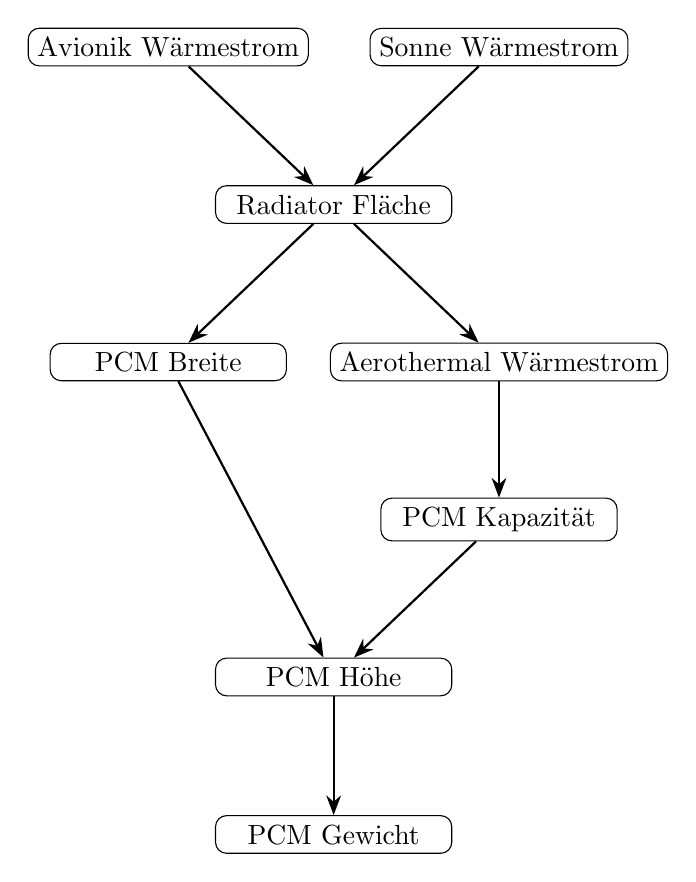
\begin{tikzpicture}[
    sibling distance=10em,
    every node/.style = {
      shape=rectangle,
      rounded corners,
      draw,
      align=center,
      minimum width=3cm
    },
    edge from parent/.style = {
      draw,
      ->,
      -{Stealth[length=0.25cm]},
      thick
    },
    arrow/.style = {
      ->,
      -{Stealth[length=0.25cm]},
      thick
    }
  ]

    % Top nodes
    \node (avionik) at (-2.1, 4) {Avionik Wärmestrom};
    \node (sonne)   at ( 2.1, 4) {Sonne Wärmestrom};

    % Radiator Fläche centered below
    \node (radiator) at (0, 2) {Radiator Fläche};

    % Children of Radiator
    \node (breite) at (-2.1, 0) {PCM Breite};
    \node (aerothermal) at (2.1, 0) {Aerothermal Wärmestrom};

    % PCM Kapazität as a separate node (not a child directly)
    \node (kapazitaet) at (2.1, -2) {PCM Kapazität};

    % PCM Höhe node below the center of breite and kapazitaet
    \node (hoehe) at (0, -4) {PCM Höhe};
    \node (gewicht) at (0, -6) {PCM Gewicht};

    % Arrows
    \draw[arrow] (avionik) -- (radiator);
    \draw[arrow] (sonne) -- (radiator);
    \draw[arrow] (radiator) -- (breite);
    \draw[arrow] (radiator) -- (aerothermal);
    \draw[arrow] (aerothermal) -- (kapazitaet);
    \draw[arrow] (breite) -- (hoehe);
    \draw[arrow] (kapazitaet) -- (hoehe);
    \draw[arrow] (hoehe) -- (gewicht);

  \end{tikzpicture}
  \caption{Dimensionierungs-Ablauf in der Vorauslegung}\label{fig:dimensionierung_ablauf}
\end{figure}

\newpage

\section{Thermales Interface}\label{thermalesInterface}

Hier gehts jetzt um wie die wärme verteilt und abtransportiert wird. Laut~\cite{Xingcun-2011} seite 35 geht die meiste Wärme in die PCB.

\newpage

\subsection{Thermal Straps}\label{thermalstraps}

Um das \ac{pcb} mit der Heatpipe zu verbinden werden Thermal Straps aus verschiedenen Materialien analysiert.
Thermal Straps sind flexible Verbindungsteile die Wärmebrücken zwischen mehreren Bauteilen gewehrleisten.
Wegen der hohe Wärmeleitzahl von \ac{pgs} und bedonders für Thermal Straps wichtigen Flexibilität, sind diese eine interessante Option.
Ein Nachteil von \ac{pgs} ist die geringe Dicke und der daraus resultierende geringe Querschnitt, welcher trotz hoher Wärmeleitzahl zu hoher Wärmestromdichte und stärkerer Temperaturerhöhung führen kann.
Im Vergleich mit herkömmlichen Materialien wie Aluminium und Kupfer soll ein Vergleich gezogen werden.

\begin{figure}[H]
  \centering
  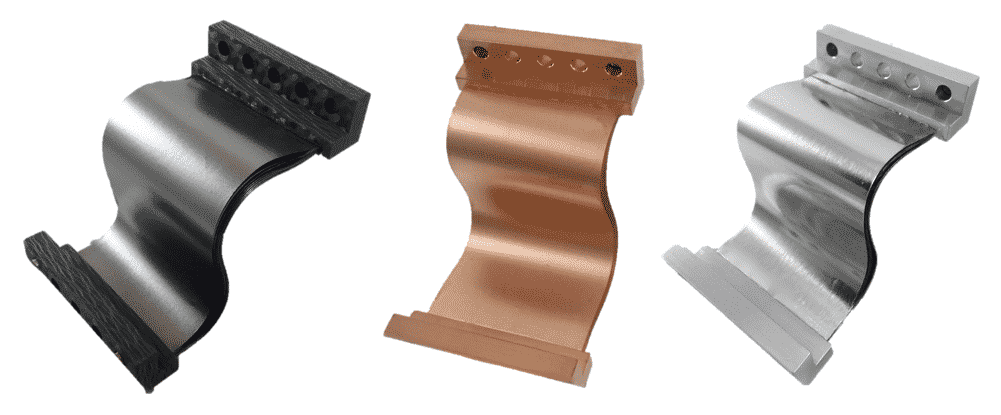
\includegraphics[width=\textwidth]{thermal_straps_commercial.png}
  \caption{Kommerzeill erhältliche Thermal Straps aus Graphen, Kupfer und Aluminium~\cite{Thermal-Straps}}\label{fig:thermalstraps_commercial}
\end{figure}

\newpage

\section{CFD}\label{cfd}

\begin{figure}[H]
    \centering
    \begin{subfigure}[t]{0.7\textwidth}
        \centering
        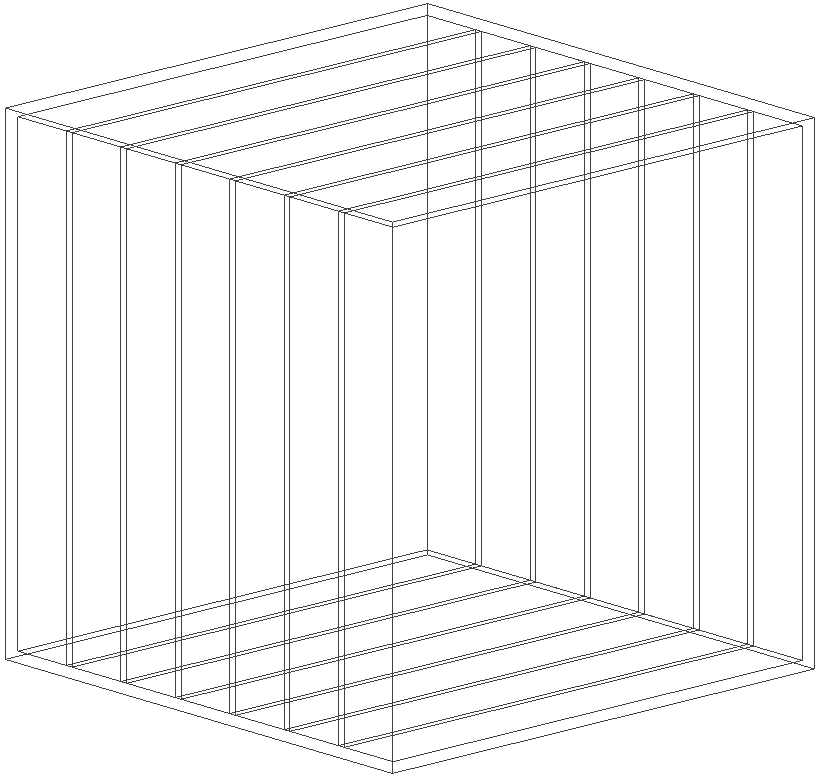
\includegraphics[height=9cm]{ansyspost/pcm/40WPCM_struktur.png}
        \caption{\ac{pcm} Struktur}\label{fig:pcm_struktur}
    \end{subfigure}
    \hfill
    \begin{subfigure}[t]{0.15\textwidth}
        \centering
        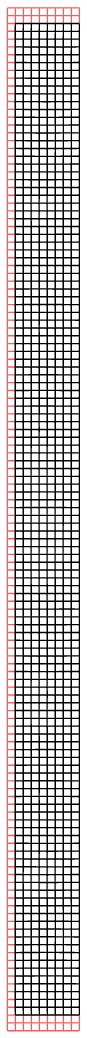
\includegraphics[height=9cm]{ansyspost/pcm/2DPCM_mesh.png}
        \caption{\ac{pcm} Mesh}\label{fig:pcm_mesh}
    \end{subfigure}
    \caption{\ac{pcm} Struktur und vereinfachtes Mesh}\label{fig:pcm_geometrien}
\end{figure}

%recoverytemperatur wahrscheinlich richtig noch recherchieren

% ----------- Diskussion & Schlussfolgerungen----------------------------------------
\newpage
\chapter{Ergebnisse}\label{chap:Ergebnisse}
Die Vorauslegungwurde mit folgenden Werten durchgeführt:\\
- Isotherm auf: \SI{38}{\celsius}\\
- Avionik Abwärme: \SI{40}{W}\\
- \SI{1}{m} Kontourlänge\\
- Radiator Emissionsgrad: \SI{0,91}{} (AZ-93)\\
- Radiator Absorptionsgrad: \SI{0,15}{} (AZ-93)\\
- Icosane PCM\\
- Trajektoriensimulation\\
- \SI{1}{\frac{kW}{m^2}} mit 50\% dutycycle durch Rotation der Rakete\\
Zu beachten ist, dass die Radiatorleistung konstant bleibt, da das System als isotherm mit einer
infinitesimalen Temperaturerhöhung über den Schmelzpunkt hinweg angenommen wird.
\section{PCM-Radiator-Hybrid}\label{sec:pcmRadiatorHybridErgebnisse}
Als nächstes sieht man Graphen
\begin{figure}[H]
  \centering
  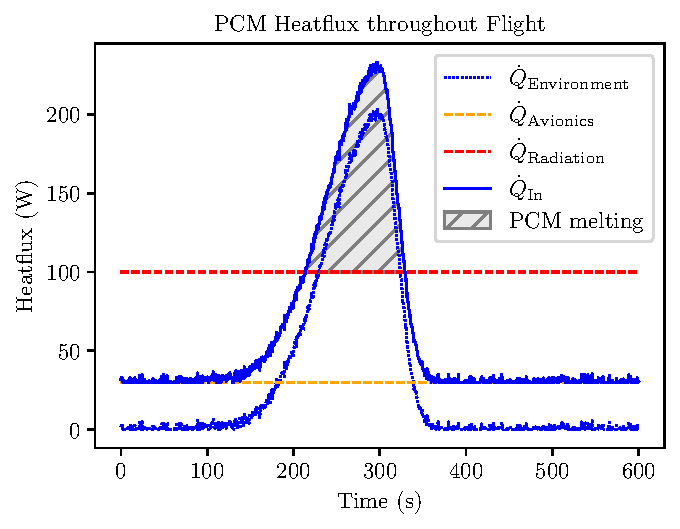
\includegraphics[width=\linewidth]{../../Code/pcm_radiator_hybrid_heatflux_during_flight.pdf}\label{fig:pcm_waermestrom_flugsimulation}
  \caption{PCM Wärmestrom während Flug}
  \includegraphics[width=\linewidth]{../../Code/re_pr_during_flight.pdf}\label{fig:re_pr_flugsimulation}
  \caption{Reynolds- und Prandtlzahl während kritischer Phase im Flug}
\end{figure}
\section{\ac{cht}}
als nächstes habe ich geschaut wo der maximale dynamische Druck erreicht wurde in der Vorauslegung. Die korrespondierenden Werte
des Flugzustandes habe ich dann als Boundery Conditions in der \ac{cfd}~Simulation genommen.
Um zu verifizieren, dass dort auch die maximale Aufheizung stattfindet, habe ich 0.5 Sekunden vorher und nachder
im Flug die BC's auch verwendet und einen Vergleich gezogen.

Maximaler dynamischer Druck: 112901.25708461029 Pa at 28.691 s
Entsprechender Flugzustand: 10244.138 m, 750.704 m/s, -51.587°C, 254.783 hPa with the corresponding air density of \SI{0.4006}{kg/m^3}

% ----------- Diskussion & Schlussfolgerungen----------------------------------------
\newpage
\chapter{Discussion and conclusions}
\label{chap:conclusion}
random zeug

Vor der Implementierung des \ac{pcm} in Hardware, sollten die Eigenschaften des vorhandenen n-Eicosan nochmal analysiert und die Ergebnisse überprüft werden.

Wenn man bessere Finnen konstruiert braucht man feineres mesh um gradienten in den wänden zu sehen


Die Vorauslegungwurde mit folgenden Werten durchgeführt:\\
- Isotherm auf: \SI{38}{\celsius}\\
- Avionik Abwärme: \SI{40}{W}\\
- \SI{1}{m} Kontourlänge\\
- Radiator Emissionsgrad: \SI{0,91}{} (AZ-93)\\
- Radiator Absorptionsgrad: \SI{0,15}{} (AZ-93)\\
- Icosane PCM\\
- Trajektoriensimulation\\
- \SI{1}{\kilo\watt\per\meter\squared} mit 50\% dutycycle durch Rotation der Rakete\\
Zu beachten ist, dass die Radiatorleistung konstant bleibt, da das System als isotherm mit einer
infinitesimalen Temperaturerhöhung über den Schmelzpunkt hinweg angenommen wird.\\
Als nächstes sieht man die Flugdaten

\section{Discussion about including pictures}


% ----------- Ausblick --------------------------------------------------------------
\newpage
\chapter{Zusammenfassung und Ausblick}
\label{chap:Ausblick}
\pagestyle{OnlySection}		% wie ganz oben definiert

Beispielliteraturverweise: 

\begin{enumerate}
	\item Fachzeitschrift
	\item Internetquelle
	\item Buch 
	\item Vorlesungsskript
\end{enumerate}

Anmerkung: Es gibt verschiedene Referenzierungsstile 

\subsection{Flüssig-Gas \ac{pcm}}
Eine weitere Methode zum Thermal-Management, die im Rahmen diese Arbeit nicht analysiert wurde, sind Flüsslig-Gas \ac{pcm}'s, welche generell signifikant höhere latente Wärmen haben,
als die hier analysierten Fest-Flüssig Varianten. Beispielsweise hat Ethanol eine Verdampfungsenthalpie von \SI{918000}{J/kg}, also fast das vierfache von Icosane, bei einer
ähnlichen Dichte. Wegen des großen Volumenanstiegs in die Gasphase von Ethanol, ist ein geschlossenes System, welches extremen Drücken standhalten müsste, eher unhandlich. Hierbei würde
das ablassen vom Ethanol in die Atmosphäre die einzige Möglichkeit sein. Da die Rakete jedoch Ethanol als Treibstoff benötigt ist ein betanken der Kühlung vor dem Start keine logistische Schwierigkeit.\\

Signifikante Probleme mit Ethanol als \ac{pcm} wären der relativ hohe Siedepunkt bei \SI{78}{\degreeCelsius}, der entweder durch Druckregelung auf $< \SI{1}{bar}$ in der oberen Atmosphäre
verringert werrden kann, oder das in Kauf nehmen einer heißer laufenden Avionik. Desweiteren verliert das System den großteil der Thermalen Masse, welche bei unvorhergesehenen Verzögerungen
des Fluges und der Recovery die Avionik schneller überhitzen lassen kann als ein geschlossenes System, in dem auch nach dem Phasenwechsel eine hohe Thermale Masse vorhanden ist.

% ----------- Literatur -------------------------------------------------------------
\newpage
\renewcommand{\bibname}{Literaturverzeichnis}

\bibliography{Bibliography/quellen.bib}
\bibliographystyle{plain}%{unsrt}{abbrv}{abbrvnat}{unsrt}

\newpage

%----------- Anhang -----------------------------------------------------------------
\chapter*{Appendix}
\label{chapter:Appendix}
\pagestyle{Appendix}
\addcontentsline{toc}{chapter}{Appendix}

\section*{Appendix A: Vorauslegung}\label{Anh:programmcode}

\begin{figure}[H]
  \centering
  \includegraphics[width=\linewidth]{../../Code/radiator_leistung.pdf}
  \caption{Radiator Leistungskonturen nach Fläche und Temperatur}\label{fig:radiator_flaeche_leistung}
\end{figure}

\begin{figure}[H]
    \centering
    \begin{subfigure}{0.9\textwidth}
        \centering
        \includegraphics[width=\linewidth]{../../Code/pcm_mass.pdf}
        \caption{Konturen der PCM Masse nach Seitenlänge und Höhe der PCM Box}\label{fig:pcm_mass}
    \end{subfigure}
    \vspace{1em}
    \begin{subfigure}{0.9\textwidth}
        \centering
        \includegraphics[width=\linewidth]{../../Code/pcm_heat_capacity.pdf}
        \caption{Konturen der PCM Latent Wärmekapazität nach Seitenlänge und Höhe der PCM Box}\label{fig:pcm_heat}
    \end{subfigure}
    \caption{PCM Auslegung}\label{fig:pcm_mass_heat}
\end{figure}

\newpage

\begin{lstlisting}[language=Python, caption={Funktionen in der hybrid.py}, label={lst:hybrid_python_pseudo}]
    # === flight data ===
    time = raw['time']  # [s]
    velocity = raw['velocity']  # [m/s]
    air_temperature = raw['air_temperature'] + 273.15  # [K]
    acceleration = raw['acceleration']
    air_pressure = raw['air_pressure'] * 100 # [Pa]

    # === constants ===
    eta_0 = 18.27e-6  # [Pa*s]
    T_0 = 291.15      # [K]
    C = 120           # [K]
    kappa = 1.4       # heat capacity ration for air
    R = 287           # [J/(kg*K)]
    c_p = 1005        # [J/(kg*K)]
    x = 1.07          # [m] radiator centerpoint (0.06 m from hull top)
    T_w = 273.15 + target_temperature # [K] PCM melting point

    # === functions ===
    def T_m(T1, T2): return (T1 + T2) / 2                                   # average temperature
    def eta(T): return eta_0 * ((T_0 + C) / (T + C)) * (T / T_0) ** (3/2)   # dynamic viscosity with surherlands formula
    def lam(T): return 2.64638e-3 + 7.326e-5 * T - 1.746e-8 * T**2          # thermal conductivity with polynomial fit
    def rho(p, T): return p / (R * T)                                       # air density
    def Pr(T): return (c_p * eta(T)) / lam(T)                               # prandtl number
    def Ma(V, T): return V / np.sqrt(kappa * R * T)                         # mach number
    def Re(V, p, T, x): return V * rho(p, T) * x / eta(T)                   # reynolds number
    def r(T): return Pr(T) ** (1/3)                                         # recovery factor
    def T_r(V, T): return T * (1 + r(T) * (kappa + 1) / 2 * Ma(V, T))       # recovery temperature
    def qdot_air(p, T, V, x, T_w):                                          # nusselt relation for wall heatflux
        Re_x = Re(V, p, T, x)
        Pr_x = Pr(T)
        Nu_x = 0.0296 * Re_x**0.8 * Pr_x**(1/3) # turbulent
        alpha = Nu_x * lam(T) / x
        return alpha * (T_r(V, T) - T_w)
    def pdyn(V, T, p): return 0.5 * rho(p, T) * V**2                        # dynamic pressure

    # === heatflux calculation ===
    Qdot_env = np.array([
        qdot_air(p, T_m(T_w, T), V, x, T_w)
        for p, T, V in zip(air_pressure, air_temperature, velocity)
    ]) * hybrid_radiator_area + (solar_flux/2 * a * hybrid_radiator_area)  # add solar flux

    Qdot_in = Qdot_env + avionics_power  # [W]

    # === fluid dynamics plot ===
    Re_plot = np.array([Re(V, p, T, x) for V, p, T in zip(velocity, air_pressure, air_temperature)])
    Pr_plot = np.array([Pr(T) for T in air_temperature])
    pdyn_plot = np.array([pdyn(V, T, p) for V, p, T in zip(velocity, air_pressure, air_temperature)])
\end{lstlisting}

\newpage

\begin{lstlisting}[language=C, caption={Vollständige \ac{pcm} \ac{udf} eicosane.c}, label={lst:udf_rest}]
    //Modified UDF of the original source: https://akamcae.com/tutorials/phase-change-material-simulation-in-ansys-fluent/
    #include "udf.h"
    #include "mem.h"

    //n-eicosane constant properties in solid phase
    #define Ros_pcm 910.0
    #define Cps_pcm 2132.4
    #define Ks_pcm 0.4248

    //n-eicosane constant properties in fluid phase
    #define Rol_pcm 769.0
    #define Cpl_pcm 2350.05
    #define Kl_pcm 0.1505

    //thermal expansion coefficient
    #define TEC 0.0009

    //solidus and liquidus temperatures of n-eicosane
    #define Ts 309.0
    #define Tl 311.0

    //reference temperature for Boussinesq's approximation
    #define Tr 310.0		//Fluent Tref must be equal to Tr

    //density of PCM
    DEFINE_PROPERTY(Ro_var_PCM,cell,thread)
    {
        double Gama, Ro_pcm;
        #if !RP_HOST
            Gama=C_LIQF(cell,thread);
            Ro_pcm=(1-Gama)*Ros_pcm+Gama*Rol_pcm;
        #endif
        return Ro_pcm;
    }

    DEFINE_SPECIFIC_HEAT(Cp_var_PCM,T,Tref,h,yi)
    {
        double Gama, Cp_pcm;
        #if !RP_HOST
            if (T<Ts) { Cp_pcm=Cps_pcm; } else if (T>=Ts&&T<=Tl)
            {
                Gama=(T-Ts)/(Tl-Ts);
                Cp_pcm=((1-Gama)*Ros_pcm*Cps_pcm+Gama*Rol_pcm*Cpl_pcm)/((1-Gama)*Ros_pcm+Gama*Rol_pcm);
            }
            else
            {
                Cp_pcm=Cpl_pcm;
            }
            *h=Cp_pcm*(T-Tref);
        #endif
        return Cp_pcm;
    }

    //thermal conductivity of n-eicosane
    DEFINE_PROPERTY(K_var_PCM,cell,thread)
    {
        double Gama, K_pcm;
        #if !RP_HOST
            Gama=C_LIQF(cell,thread);
            K_pcm=(1-Gama)*Ks_pcm+Gama*Kl_pcm;
        #endif
        return K_pcm;
    }

    //dynamic viscosity of PCM with fit
    DEFINE_PROPERTY(Mu_var_PCM,cell,thread)
    {
        double Temp,Mu_pcm;
        #if !RP_HOST
            Temp=C_T(cell,thread);
            Mu_pcm=(9*pow(10.,-4)*pow(Temp,2)-0.6529*Temp+119.94)*pow(10.,-3);
        #endif
        return Mu_pcm;
    }

    DEFINE_SOURCE(Boussinesq_momentum_source,cell,thread,dS,eqn)
    {
        double Temp, source, acc;
        Temp=C_T(cell,thread);

        double t = CURRENT_TIME;

        if (t < 20)
            acc = 34.81;
        else if (t < 50)
            acc = 109.81;
        else if (t < 150)
            acc = 19.62;
        else
            acc = 9.81;

        source=-Rol_pcm*acc*TEC*(Temp-Tr); //negative for -Y down
        dS[eqn]=-Rol_pcm*acc*TEC; //negative for -Y down
        return source;
    }
\end{lstlisting}

% \begin{lstlisting}[language=python, caption={setup.json}, label={lst:setup.json}]
% {
%     "devmode": 0,
%     "avionics_power": 40,
%     "target_temperature": 36.85,
%     "emittance": 0.91,
%     "absorptance": 0.15,
%     "solar_flux": 1000,
%     "trajectory_data_path": "blast.csv"
% }
% \end{lstlisting}

% \begin{lstlisting}[language=python, caption={results.json}, label={lst:results.json}]
% {
%     "hybrid_radiator_area": 0.0996163285294786,
%     "hybrid_radiator_power": 47.471224639710904,
%     "hybrid_capacity_sim": 188087.64535959047,
%     "hybrid_capacity_nu": 626817.5705502237,
%     "pcm_capacity": 48000.0,
%     "hybrid_H_sim": 0.013188203298524867,
%     "hybrid_m_sim": 1.6535028624398134,
%     "hybrid_H_nu": 0.03928567591747304,
%     "hybrid_m_nu": 4.255679378864365,
%     "normal_L_solution": 0.06748627883089094,
%     "normal_m_solution": 0.346609735620966
% }
% \end{lstlisting}

% \begin{lstlisting}[language=python, caption={main.py}, label={lst:main.py}]
% import subprocess

% subprocess.run(["python", "radiator.py"])
% subprocess.run(["python", "hybrid.py"])
% subprocess.run(["python", "pcm.py"])
% subprocess.run(["python", "pcmProperty.py"])
% subprocess.run(["python", "post.py"])
% \end{lstlisting}

% \begin{lstlisting}[language=python, caption={radiator.py}, label={lst:radiator.py}]
% # This Program calculates the steady-state equation for a grey body radiator

% import numpy as np
% import json
% from scipy.constants import Stefan_Boltzmann, pi
% import matplotlib.pyplot as plt
% import matplotlib as mpl



% # === configuration ===
% # load data from setup.json
% try:
%     with open("setup.json", "r", encoding="utf-8") as f:
%         data = json.load(f)
% except FileNotFoundError:
%     print("setup.json not found. Exiting.")
%     exit()
% except json.JSONDecodeError:
%     print("setup.json is empty of invalid. Exiting.")
%     exit()

% DEVELOPMENT_MODE = data["devmode"]
% avionics_power = data["avionics_power"] # W
% e = data["emittance"]
% a = data["absorptance"]
% solar_flux = data["solar_flux"] # W*m^-2
% target_temperature = data["target_temperature"]

% # Set global matplotlib style
% mpl.rcParams.update({
%     "figure.figsize": (4.9, 3.5),
%     "font.size": 11.0,
%     "font.family": "serif",
%     "font.serif": ["cmr10"],
%     "axes.titlesize": "medium",
%     "figure.titlesize": "medium",
%     "text.usetex": not DEVELOPMENT_MODE,
%     "text.latex.preamble": r"\usepackage{amsmath}\usepackage{amssymb}\usepackage[=v2]{siunitx}\usepackage[utf8]{inputenc}"
% })



% # === Equations ===
% rho_alu = 2700 # kg/m^3
% T_target = 273.15+target_temperature # target temperature

% # Define temperature in Celsius for plotting, and convert to Kelvin
% temp_C = np.linspace(0, 100, 100) # ^\circ C
% A = np.linspace(0.01*0.01, 0.3*0.3, 100) # Area [m$^2$]

% A_grid, T_C_grid = np.meshgrid(A, temp_C)
% T_K_grid = T_C_grid + 273.15  # Convert Celsius to Kelvin for calculation

% # Stefan-Boltzmann radiation formula
% phi_radiation = (A_grid * e * Stefan_Boltzmann * T_K_grid**4) # [W]



% # === Target result ===
% hybrid_radiator_area = (avionics_power) / ((e * Stefan_Boltzmann * T_target**4)-(solar_flux/2)*a) # [m^2] necessary radiator area to get rid of avionics- and solarheatflux
% hybrid_radiator_power = hybrid_radiator_area*e*Stefan_Boltzmann*T_target**4 # [W] total out-heatflux of radiator

% # Putting Data into result.json
% with open("result.json", "w", encoding="utf-8") as f:
%     json.dump({}, f, indent=4)  # clear result.json as this is the first write in the programm chain

% data = {
%     "hybrid_radiator_area": hybrid_radiator_area,
%     "hybrid_radiator_power": hybrid_radiator_power
% }

% with open("result.json", "w", encoding="utf-8") as f:
%     json.dump(data, f, indent=4)



% # === Plotting ===
% # Plot
% fig1 = plt.figure(figsize=(8, 6))
% contour = plt.contour(A_grid, T_C_grid, phi_radiation, levels=20, colors='black')
% #plt.colorbar(contour, label='W\"arme [W]')   # colorful contours
% plt.clabel(contour, inline=True, levels=contour.levels[::2], fontsize=10, fmt='%1.1f [W]') # levels makes every second contour have a label
% plt.xlabel(r"Fl\"{a}che [m$^2$]")
% plt.ylabel(r"Temperatur [^\circ C]")
% plt.grid(True)

% if DEVELOPMENT_MODE:
%     plt.title(r"Radiator W\"armestrahlung nach Fl\"{a}che und Temperatur")

% # Save it if not in dev mode
% if not DEVELOPMENT_MODE:
%     fig1.savefig("radiator_leistung.pdf", bbox_inches="tight")

% if DEVELOPMENT_MODE:
%     plt.show()
% \end{lstlisting}

\section*{Appendix B: Simulation}\label{Anh:simulation}

\begin{figure}[H]
    \centering

    \begin{subfigure}{\textwidth}
        \centering
        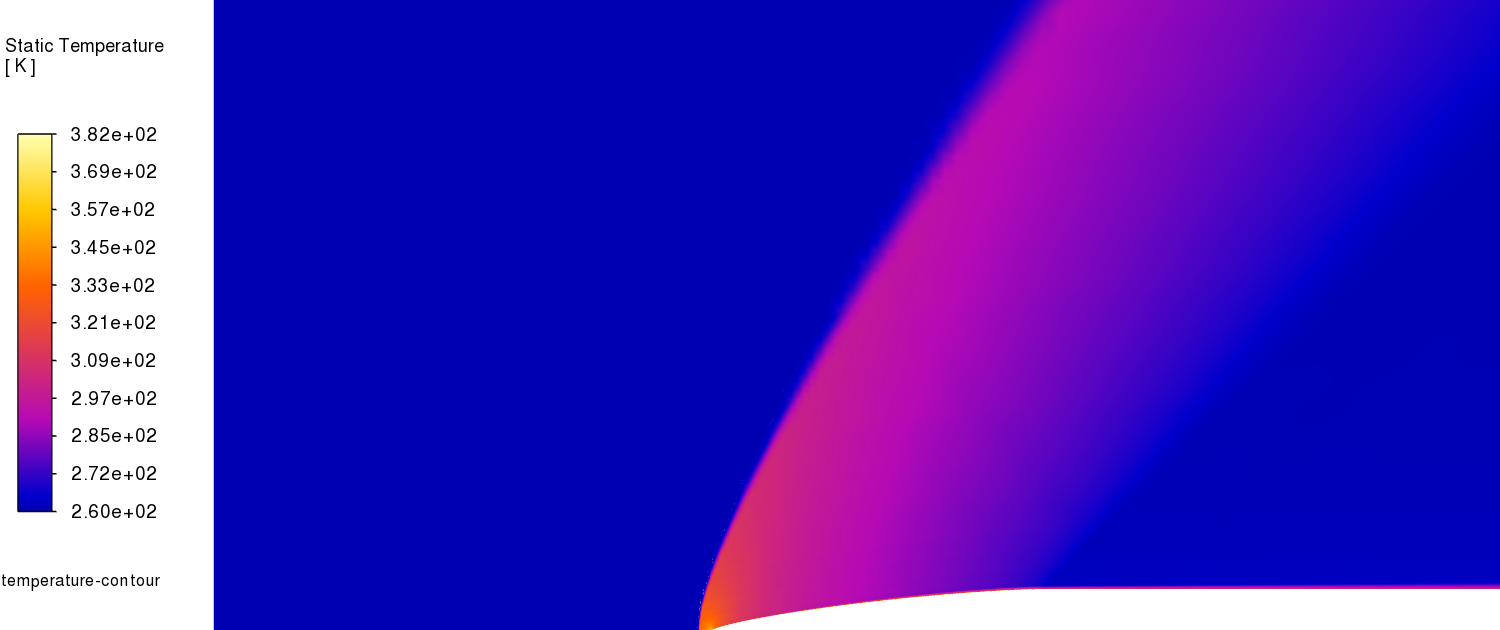
\includegraphics[height=0.23\textheight]{ansyspost/airflow/maxQminus10-temperature-contour.png}
        \caption{\ac{maxq} -\SI{10}{\second}}
        \label{fig:maxQminus10_temp_contour}
    \end{subfigure}

    \begin{subfigure}{\textwidth}
        \centering
        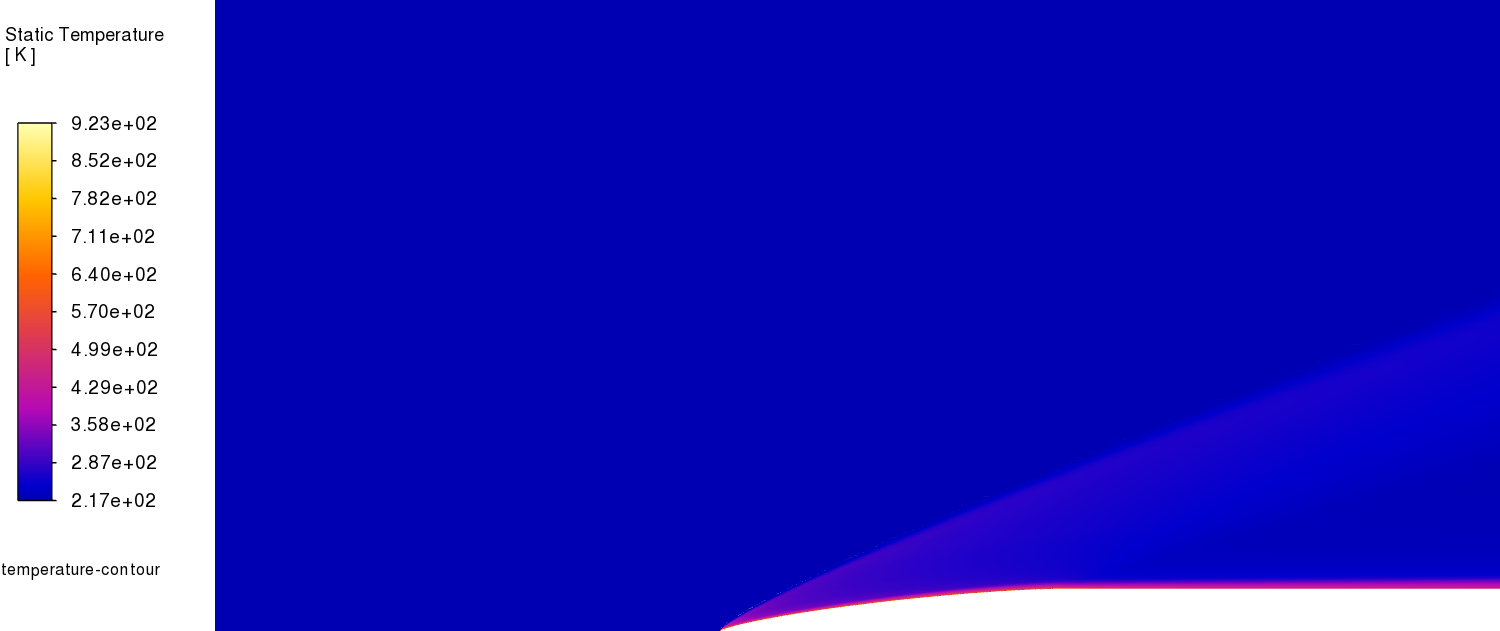
\includegraphics[height=0.23\textheight]{ansyspost/airflow/maxQplus10-temperature-contour.png}
        \caption{\ac{maxq} +\SI{10}{\second}}
        \label{fig:maxQplus10_temp_contour}
    \end{subfigure}

    \begin{subfigure}{\textwidth}
        \centering
        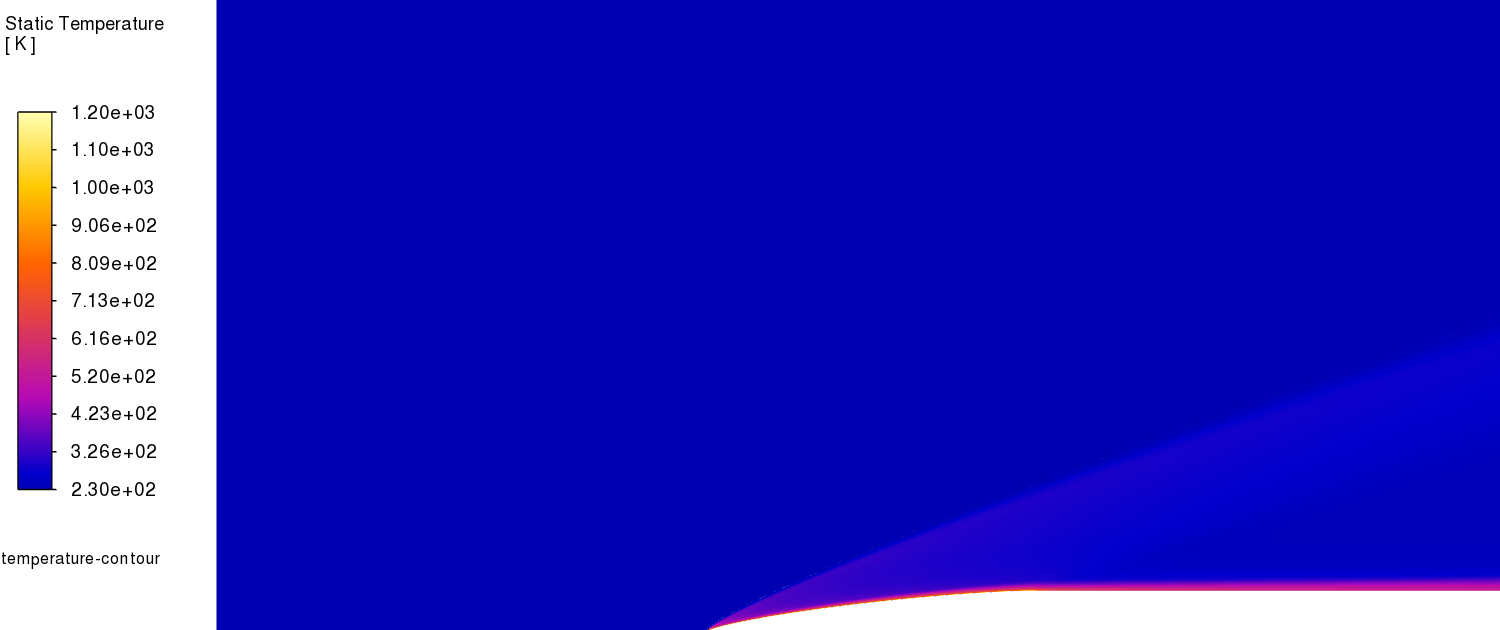
\includegraphics[height=0.23\textheight]{ansyspost/airflow/maxQplus20-temperature-contour.png}
        \caption{\ac{maxq} +\SI{20}{\second}}
        \label{fig:maxQplus20_temp_contour}
    \end{subfigure}

    \caption{Statische Temperaturkontur der Luft}
    \label{fig:airflow_temp_contour_continued}
\end{figure}

\begin{figure}[H]
    \centering

    \begin{subfigure}{\textwidth}
        \centering
        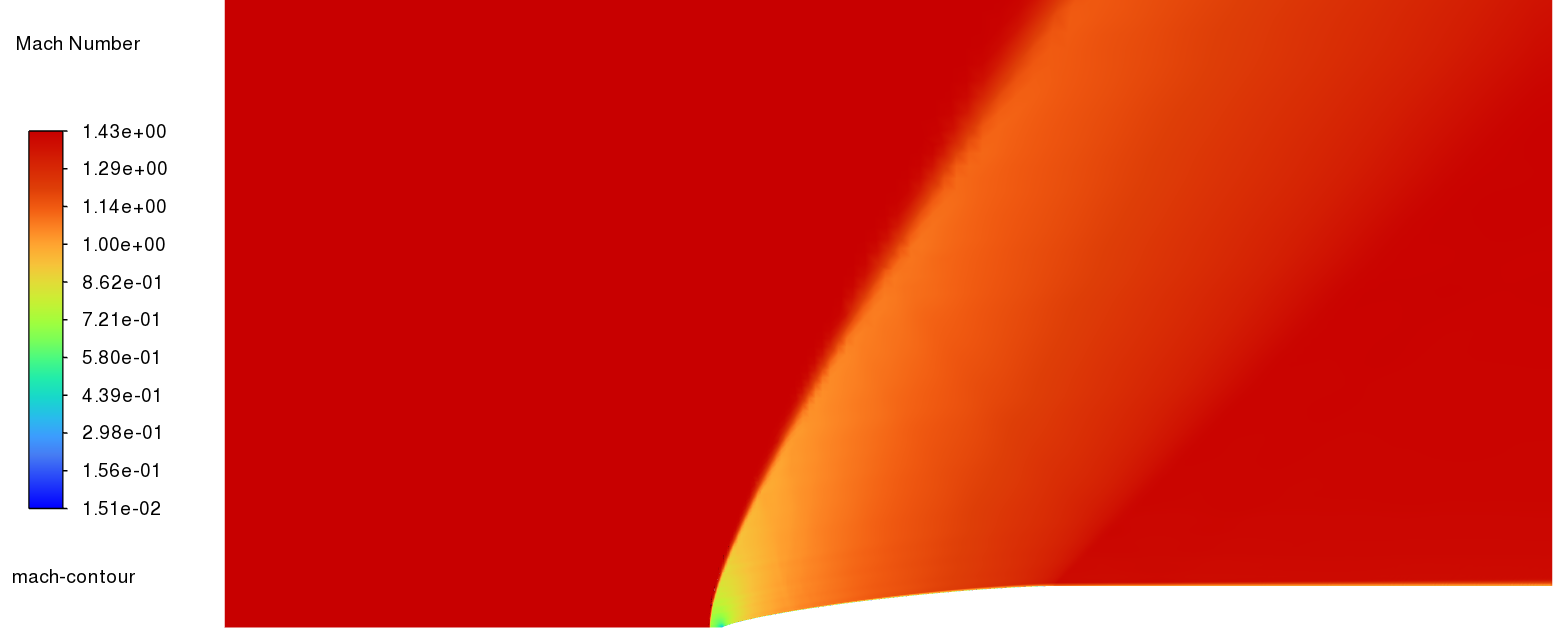
\includegraphics[height=0.23\textheight]{ansyspost/airflow/maxQminus10-mach-contour.png}
        \caption{\ac{maxq} -\SI{10}{\second}}
        \label{fig:maxQminus10_mach_contour}
    \end{subfigure}

    \begin{subfigure}{\textwidth}
        \centering
        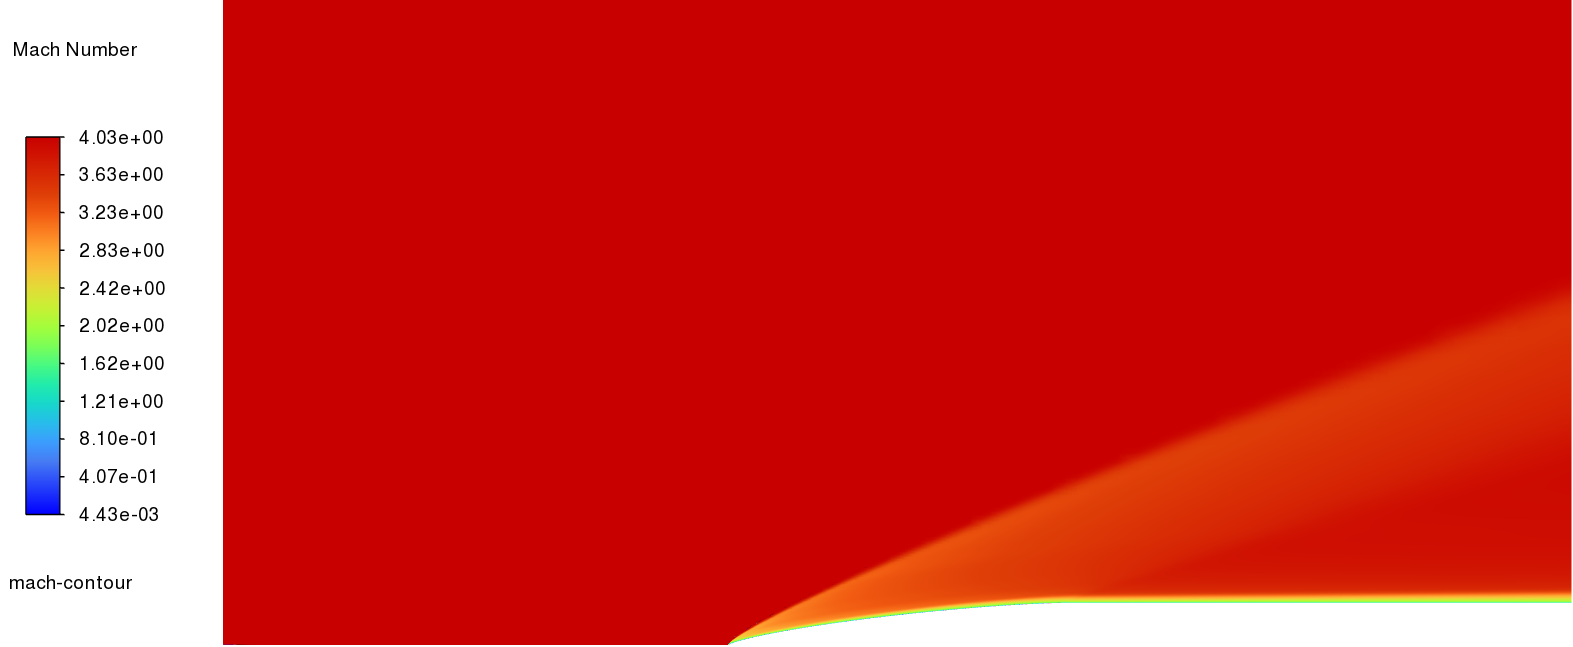
\includegraphics[height=0.23\textheight]{ansyspost/airflow/maxQplus10-mach-contour.png}
        \caption{\ac{maxq} +\SI{10}{\second}}
        \label{fig:maxQplus10_mach_contour}
    \end{subfigure}

    \begin{subfigure}{\textwidth}
        \centering
        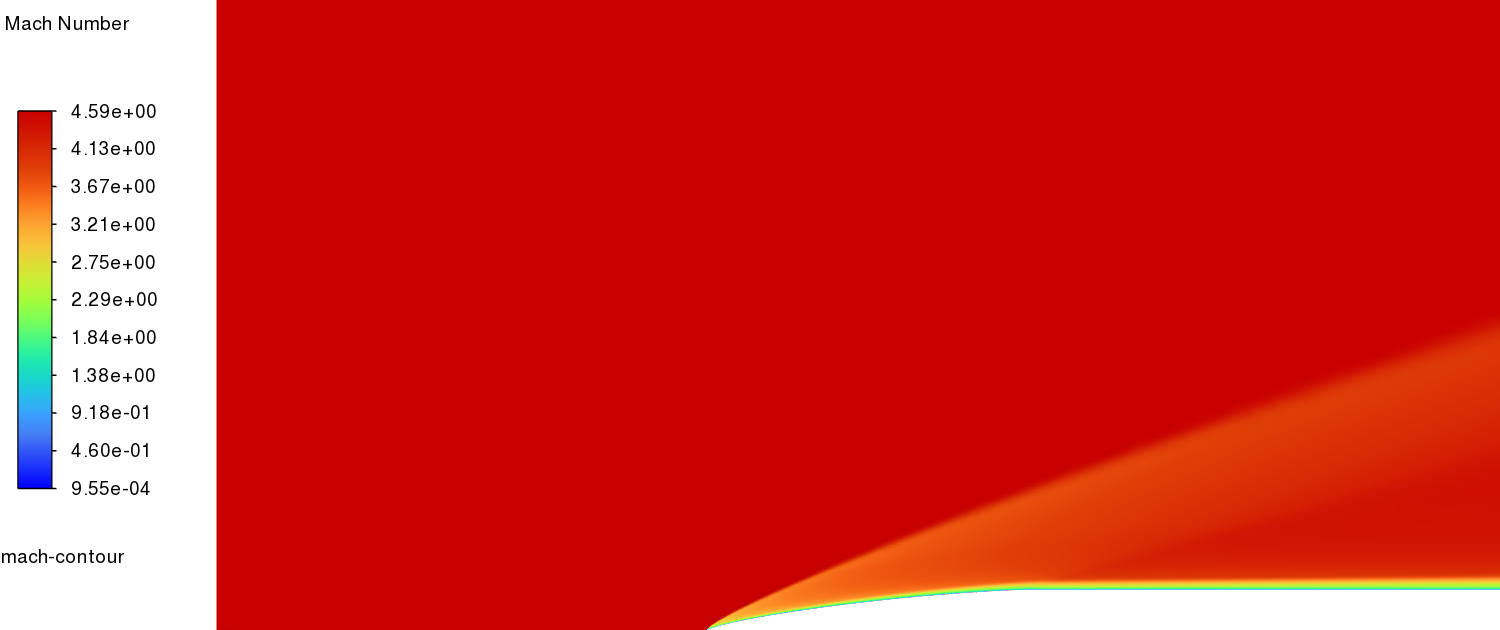
\includegraphics[height=0.23\textheight]{ansyspost/airflow/maxQplus20-mach-contour.png}
        \caption{\ac{maxq} +\SI{20}{\second}}
        \label{fig:maxQplus20_mach_contour}
    \end{subfigure}

    \caption{Machzahlkontur der Luft}
    \label{fig:airflow_mach_contour_continued}
\end{figure}

\begin{figure}[H]
    \centering

    \begin{subfigure}[t]{0.14\textwidth}
        \centering
        \raisebox{1\height}{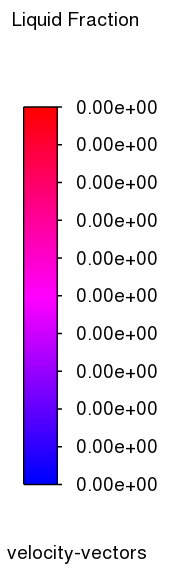
\includegraphics[height=0.2\textheight]{ansyspost/pcm/vector-legend.png}}
    \end{subfigure}%
    \hspace{2mm}% extra space between legend and first image
    \begin{subfigure}[t]{0.2\textwidth}
        \centering
        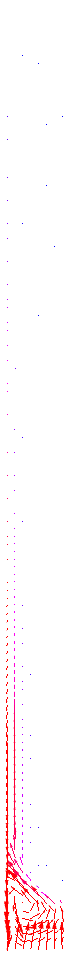
\includegraphics[height=0.7\textheight]{ansyspost/pcm/velocity-vector-300.png}
        \caption{\SI{300}{\second}}\label{fig:velocity_vector_300}
    \end{subfigure}%
    \begin{subfigure}[t]{0.2\textwidth}
        \centering
        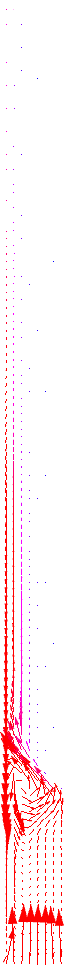
\includegraphics[height=0.7\textheight]{ansyspost/pcm/velocity-vector-600.png}
        \caption{\SI{600}{\second}}\label{fig:velocity_vector_600}
    \end{subfigure}%
    \begin{subfigure}[t]{0.2\textwidth}
        \centering
        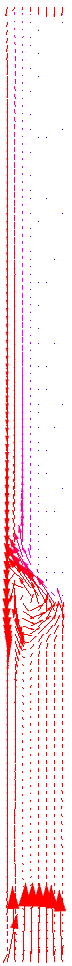
\includegraphics[height=0.7\textheight]{ansyspost/pcm/velocity-vector-900.png}
        \caption{\SI{900}{\second}}\label{fig:velocity_vector_900}
    \end{subfigure}%
    \begin{subfigure}[t]{0.2\textwidth}
        \centering
        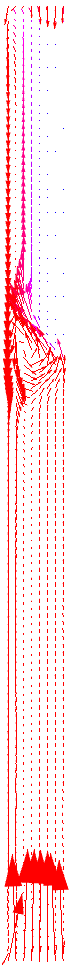
\includegraphics[height=0.7\textheight]{ansyspost/pcm/velocity-vector-1200.png}
        \caption{\SI{1200}{\second}}\label{fig:velocity_vector_1200}
    \end{subfigure}
    \caption{Konturen der statischen Temperatur. Die Legende bezieht sich auf~\ref{fig:velocity_vector_1200}}\label{fig:pcm_static_temperature_kontur}
\end{figure}

%------------------------------------------------------------------------------------
\end{document}
